\chapter{Realisation}


\section{Overview}

As explains above in the state of the art and in the figure\ref{tableau_comparatif} each approach has its advantages and its disadvantages. That is why in our solution we tried to take the better of the two worlds. We stylize the 3D scene in image space (screen space) but with all the information about the 3D object and the camera (camera matrices, position, normals, tangents, UV coordinates, distance from the camera). This solution permits to apply something like 2D images on the screen so have a good \textit{flatness} while keeping the information on the silhouettes, the orientation, the depth, etc. This solution permits also to easily integrate the stylizing of a scene in a pipeline rendering because it can be done at the end during the post-processing rendering pass. \newline

We chose to use mark based methods to stylize our scene because texture based methods in image space give a poor variety of styles as said in the work of Bénard et al.\cite{benard_dynamic_2009}. This mark based method implies to decide where in the image the splats will be drawn. In our problem, the goal is to anchor these splats with the objects in order to have the same motion for the splats and the object. This avoid the problem of \textit{shower door effect} and ensure the good \textit{motion coherence}. So we needed anchor points depending on the position of our object. Therefore in our approach, we used procedural noise\cite{perlin_improving_2002} as a texture of our 3D object. The procedural noises are easy to implement, fast to compute and easy to manipulate. Like every texture computed in object space, it has a good motion coherence. Each value different of zero of this texture represents an anchor point for a splat.


\section{Procedural noise and fractalization}

\begin{figure}
    \begin{center}
    
\includegraphics[scale=0.2]{images/PerlinNoise2d.png}
    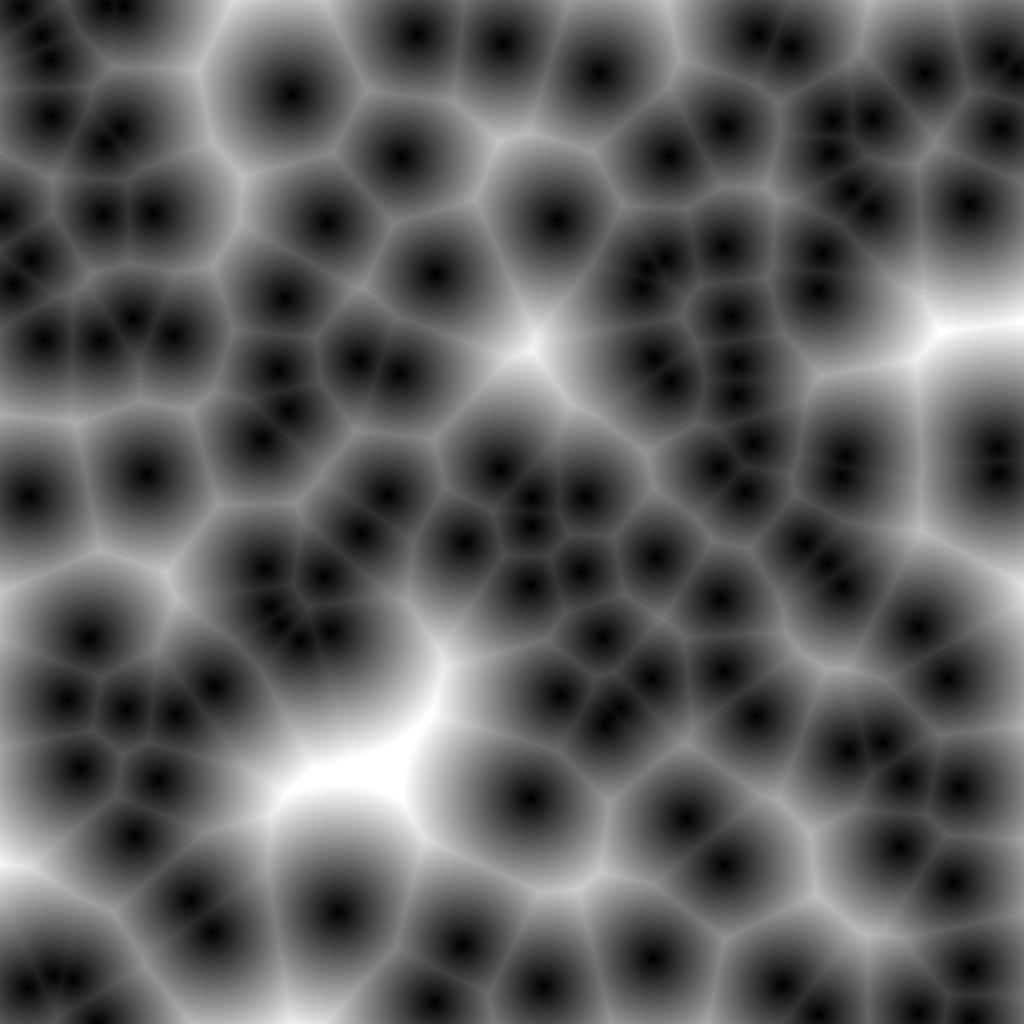
\includegraphics[scale=0.1]{images/WorleyNoise2d.jpg}
    \end{center}
    \caption{Examples of procedural texture: \textit{left using perlin noise, right using worley noise}}
    \label{procedural_texture}
\end{figure}

% Description of procedural noise

We compute procedural texture in order to create anchor points. Procedural noises are \textit{pseudorandom} gradient of grid point. In computer grapchis, they are usually used in 2d \ref{procedural_texture} as an image or in 3d for texturing a 3d object, in our case we use it in 3d. This texture are computed from procedural noise with a mathematical process. There exist many procedural noise such as Perlin noise, Worley noise, Gabor noise, Value noise, Gradient noise, etc. In order to map the procedural texture to the 3d object, we compute it with the vector position of each vertex of the object. The frequency of a noise control how many details there is in the texture. With a Worley noise, increasing the frequency will increase the number of black area in the texture.

% how we use it

\begin{figure}
    \begin{center}
    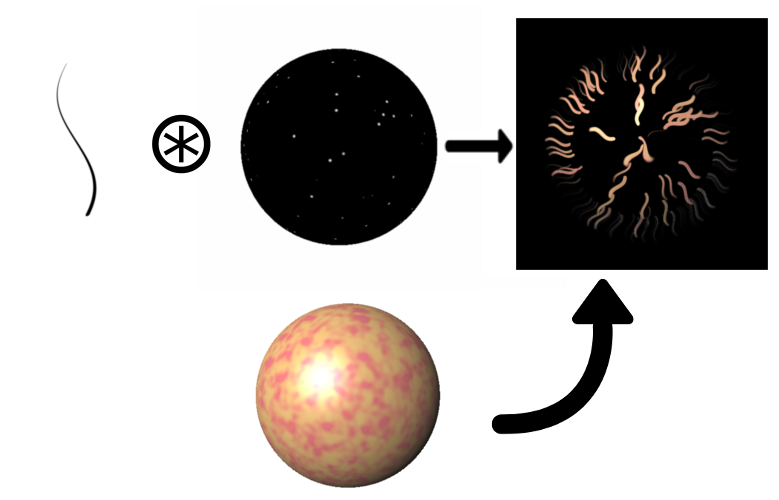
\includegraphics[scale=0.6]{images/noise/addition.png}
    \end{center}
    \caption{Usage of procedural texture to anchor splats}
    \label{procedural_noise_anchor}
\end{figure}

In our case we used the procedural texture to anchor the splat. For each pixel of the final image we "paste" a splat if the current pixel correspond to black pixel in the procedural texture the splat is not displayed (see Figure \ref{procedural_noise_anchor}). Thanks to this mechanism we can control the density of splat in the image.


% Add fractalization

\textbf{Fractalization}
 Bénard et \textit{al.}\cite{benard_dynamic_2010} use the same principle but with procedural textures. They create multiple noises with different frequency and combine them playing with transparency. Moreover, they overlap the noise to make an impression of infinite zoom effect (like in this example: \href{https://www.shadertoy.com/view/XlBXWw?fbclid=IwAR1fU2JxQzXtks1ZcmVmzrHiv646G8w2gWceeiV-UToeFkAFMQ2NecbsGGs}{ShaderToy}). With this method patterns of the texture have an almost constant size regardless of the size of the object but it can create small problems of \textit{temporal continuity}. In our method, we will use this technique of fractalization of a procedural noise. \newline

\section{Splatting}


\section{Stylization}
